\section{Methodology}

This section describes some of the theory and methods involved in this work. Firstly, we provide analytical expressions for the degree-2 tidal potential in section \ref{subsec:pot}. The governing equations of the numerical model are then discussed in section \ref{subsec:LTE}. Following this, a description of the equations discretisation and the numerical scheme required to solve them are outlined in section \ref{subsec:model}.

\subsection{Laplace Tidal Equations \label{subsec:LTE}}

The equations of motion and mass conservation that describe ocean flow in the shallow water limit are called the Laplace Tidal Equations (LTE) (also known as the shallow water equations) \citep{lamb1932hydrodynamics}. The main assumption in their derivation is that radial (vertical) ocean flow is negligible when compared to lateral flow. This is indeed a good approximation for global oceans, where lateral flow spans a much greater distance than the depth of the ocean. The conservation of mass (eq. \ref{eq:mass}) and momentum (eq. \ref{eq:mom}) that make up the LTE, including both Rayleigh and bottom friction, are given as \citep{sears1995tidal,tyler2008strong,matsuyama2014tidal}:

%Adds vertical space between equations
%\setlength{\jot}{8pt}
%environment centres all equations

\vspace{-0.5cm}
\begin{gather}
\partial_t \eta + \nabla \cdot \left(h \bm{u}\right) = 0\, , \label{eq:mass}\\
\begin{aligned} 
\partial_t \bm{u} + 2 \bm{\Omega} \times \bm{u} + \alpha\bm{u} + \frac{c_D}{h} \left|\bm{u}\right| \bm{u}  + g \nabla \eta \\ = (1 + k_2 - h_2) \nabla U_2 \, . \label{eq:mom}\\
\end{aligned} 
\end{gather}

Equation \ref{eq:mass} consists of two terms. The first is the time rate of change of vertical sea surface displacement about some equilibrium level. $\eta$ denotes this displacement. The second term represents the divergence of the surface velocity vector, $\bm{u} \equiv (u, v)$, where $u$ and $v$ are the eastward and northward velocity components respectively. In our calculations, we assume the ocean's undisturbed depth, $h$, to be constant. 

\begin{figure*}[t]
\centering
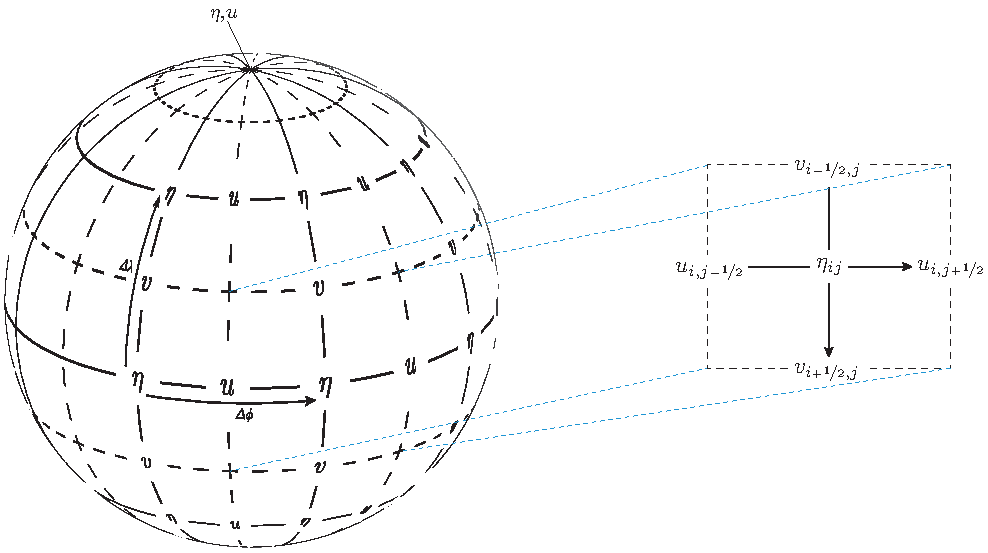
\includegraphics[width=0.8\linewidth]{Figures/GridDiagram}
\caption{The staggered grid structure used in ODIS. A single cell is show on the right of the figure, where surface displacement, $\eta$, represents a cell centered quantity. $u$ velocity nodes are staggered eastward of $\eta$, whereas $v$ velocity nodes are staggered southwards. Both $u$ and $v$ are defined at the cell walls. Lines of meridian merge to singularities at the poles, where both a single $u$ and $\eta$ point are stored.\label{fig:grid}}
\end{figure*}

The term on the right hand side of Equation \ref{eq:mom} is an applied force per unit mass. $\nabla U_2$ is the gradient of the degree-2 tidal potential (discussed in section ...). It is multiplied by Love's reduction factor involving the degree-2 tidal Love numbers, $k_2$ and $h_2$. Love's first number, $k_2$, is a proportionality constant accounting for the additional tidal potential due to the elastic redistribution of mass on the satellite. $h_2$, the second Love number, accounts for the tidal potential arising from solid body surface displacement of the satellite \citep{love1911some}.

The time derivative of velocity is given by the first term on the left hand side of the momentum equation. It is balanced by four other acceleration per unit mass terms on the left hand side. The first of these terms is the coriolis acceleration per unit mass, where $\Omega$ is the satellite's rotational angular velocity. Rayleigh and bottom friction are described in the next two terms, where $\alpha$ and $c_D$ are the Rayliegh (linear)and bottom (quadratic) friction coefficients respectively \citep{sears1995tidal,chen2013tidal}. The last term on the right hand side of Equation \ref{eq:mom} is the gravitational restoring acceleration per unit mass. It acts to balance changes in sea surface displacement, given by the gradient of equilibrium displacement, $\nabla \eta$ .

\subsection{Tidal Potential \label{subsec:pot}}

Finite eccentricity and obliquity cause libration of the satellite's tidal bulge in longitude and latitude, respectively. It is this libration that primarily induces ocean flow. We therefore find it convenient to split the full degree two tidal potential into its two primary components, the eccentricity and obliquity tides:
\begin{align}
U_2 &= U_{ecc} + U_{obliq}\, . \label{eq:U_2}
\end{align}
The eccentricity and obliquity tide can be expressed as \citep{tobie2005tidal,tyler2011tidal,matsuyama2014tidal},
\begin{multline}
U_{ecc} = \Omega^2 r^2 e \left\lbrace - \frac{3}{2} P_{20}\left(\cos\theta\right) \cos \left(\Omega t \right) + \frac{1}{8} P_{22}\left( \cos\theta\right) \right. \\ 
\times \left. \vphantom{\frac{1}{8}} \left[7 \cos \left(2 \phi - \Omega t \right) - \cos \left(2 \phi + \Omega t\right) \right] \right\rbrace, \label{eq:U_ecc}
\end{multline} and,
\begin{multline}
U_{obliq} = \frac{1}{2}\Omega^2 r^2 \theta_0 P_{21}\left(\cos\theta\right)\\
\times \left[ \cos \left(\phi - \Omega t \right) - \cos \left( \phi + \Omega t\right) \right] \, ,\label{eq:U_obliq}
\end{multline}
where $r$ is the satellite's radius, $e$ is its eccentricity, and $\theta_0$ is the obliquity in radians. Co-latitude and longitude are given as $\theta$ and $\phi$ respectively. $P_{lm}$ represent the associated Legendre function of degree $l$ and order $m$. The eccentricity tide in Equation \ref{eq:U_ecc} can be further split into the two terms on its right hand side. From the left, these terms represent the eccentricity-radial ($U_{20}$) and eccentricity-libration ($U_{22}$) tides respectively, as described by \citet{tyler2011tidal}. We can therefore rewrite equation \ref{eq:U_2} as $U_2 = U_{20} + U_{21} + U_{22}$.

The derivatives of equations \ref{eq:U_ecc} and \ref{eq:U_obliq}, required to solve the LTE, are given in the appendix.

\subsection{Numerical Model \label{subsec:model}}

In this section we outline our numerical model Ocean Dissipation in Icy Satellites (ODIS). In its current form, ODIS is based extensively on the models discussed in and developed by \citet{zahel1973diurnalk,zahel1978influence} and \citet{sears1994tidal,sears1995tidal}. Firstly, we provide a description of the numerical grid design. We then give an overview of the finite difference scheme itself, before finishing on limitations of the finite difference scheme and grid choice.

\subsubsection{Discretized Grid \label{subsec:grid}}

We employ a fixed latitude-longitude grid for our numerical simulations, defined in a spherical coordinate system. The grid is constructed in a staggered manner, meaning that velocity nodes are placed to the east and south of their parent displacement nodes. This is illustrated in Figure \ref{fig:grid}, where we define $u$ and $v$ as the eastward and northward velocity components, respectively ($\bm{u} \equiv \left(u,v\right))$. $\Delta \lambda$ is the latitude grid spacing, whereas $\Delta \phi$ is the longitude grid spacing. A staggered approach is reasonably common in CFD problems as it avoids oscillations that grow in the solution by calculating derivatives \textit{between} grid points, rather than over them. This is discussed further in section \ref{subsec:fd_expan}.

As is clear from Figure \ref{fig:grid}, lines of meridian all converge to single points at either pole. As a result, the model is forced to go from $m$ points immediately surrounding the pole, to merely a single point at either pole. Accordingly, both single values of $\eta$ and $u$ are stored at each pole. This approach slightly differs from \citet{sears1995tidal}, whom stored only a single $\eta$ value at the poles.

ODIS stores three separate 2D arrays for $\eta$, $u$ and $v$. They are accessed in a parent-child configuration, whereby the velocity nodes immediately east and south of a displacement node are the children to their parent $\eta$. Both $u$ and $v$ at the southern and eastern walls of the cell in Figure \ref{fig:grid} are children to the central $\eta$ node. This fact is of little unimportance to the model's computations, but does lend some insight into the model's infrastructure.

\subsubsection{Finite Difference Expansions \label{subsec:fd_expan}}

In order to solve the LTEs, we expand equations \ref{eq:mass} and \ref{eq:mom} in a semi-implicit finite difference scheme in spherical coordinates, following \citep{sears1995tidal}. By expanding $\bm{u}$ into its components, the momentum equation becomes,

\vspace{-0.6cm}
\begin{multline}
u_{ij}^{t+1} \approx  \left[ \,2 \Omega \bar{v}_{ij} \sin{\lambda_i} \vphantom{\frac{c_D}{h}\sqrt{\left(u_{ij}^{t}\right)^2}} - \alpha u_{ij}^{t} \right. \\ 
- \frac{c_D}{h}\sqrt{\left(u_{ij}^{t}\right)^2 + \left(\bar{v}_{ij}^{t}\right)^2}\cdot\left(u_{ij}^{t}\right)^2 - \frac{g}{R \cos{\lambda_i}} \frac{\partial \eta_{ij}^{t}}{\partial \phi_j} \\  
+ \left.\left(1 + k_2 - h_2\right) \frac{1}{R \cos{\lambda_i}} \frac{\partial U_{2,ij}^{t}}{\partial \phi_j} \right]  \Delta t + u_{ij}^{t} \, , \label{eq:momu_fd}
\end{multline}
\vspace{-0.6cm}
\begin{multline}
v_{ij}^{t+1} \approx  \left[ \,-2 \Omega \bar{u}_{ij} \sin{\lambda_i} \vphantom{\frac{c_D}{h}\sqrt{\left(u_{ij}^{t}\right)^2}} - \alpha v_{ij}^{t} \right. \\ 
- \frac{c_D}{h}\sqrt{\left(\bar{u}_{ij}^{t}\right)^2 + \left(v_{ij}^{t}\right)^2}\cdot\left(v_{ij}^{t}\right)^2 - \frac{g}{R} \frac{\partial \eta_{ij}^{t}}{\partial \lambda_i} \\  
+ \left.\left(1 + k_2 - h_2\right) \frac{1}{R} \frac{\partial U_{2,ij}^{t}}{\partial \lambda_i} \right]  \Delta t + v_{ij}^{t} \, , \label{eq:momv_fd}
\end{multline}

\noindent and the mass conservation equation becomes, 
\begin{equation}
\eta_{ij}^{t+1} \approx 
-\frac{h}{R \cos{\lambda_i}}\left(
\frac{\partial \left(v_{ij}^{t+1} \cos{\lambda_i}\right)}{\partial	\lambda_i}  
+\frac{\partial u_{ij}^{t+1}}{\partial	\phi_j}\right)
\Delta t
+ \eta_{ij}^{t}\, . \label{eq:mass_fd}
\end{equation}

Latitude and longitude are denoted by $\lambda$ and $\phi$ respectively. $i$ and $j$ represent the $i\text{th}$ and $j\text{th}$ latitude and longitude positions within the grid. The time index is given by $t$, and $\Delta t$ represents the time-step. Overbars correspond to averages, a necessity given the staggered nature of the grid.

All derivatives of the degree-2 tidal potential (equations \ref{eq:U_ecc} and \ref{eq:U_obliq}) have analytical solutions, and thus do not require further finite difference expansions. These derivatives are given in the appendix. Derivatives of all other quantities, however, do require further expansion. The expansions take the general form of either,

\begin{align}
\frac{\partial w_{ij}}{\partial \lambda} &\approx \frac{w_{i+\nicefrac{1}{2},j} - w_{i-\nicefrac{1}{2},j}}{\Delta \lambda} \, , \label{eq:gen1}
\shortintertext{or, }
\frac{\partial w_{ij}}{\partial \phi} &\approx \frac{w_{i,j+\nicefrac{1}{2}} - w_{i,j-\nicefrac{1}{2}}}{\Delta \phi} \, , \label{eq:gen2}
\end{align}

\noindent where $w$ represents $u$, $v$ or $\eta$.

Examining equations \ref{eq:gen1} and \ref{eq:gen2} reveals that each derivative is evaluated halfway between the grid points where $w$ is stored. Consequently, any derivative of $w$ is calculated at the grid position held by a different function. For example, $\partial_\phi u_{ij}$ is always evaluated at the position held by $\eta_{ij}$ as $u_{i,j-\nicefrac{1}{2}}$ and $u_{i,j+\nicefrac{1}{2}}$ lie to the left and right of $\eta_{ij}$,  respectively. This is shown in Figure \ref{fig:grid}.

\subsubsection{Numerical Scheme}

ODIS begins its calculations by determining the mass of each volume element in the initial ocean, whether it be undisturbed or from some other initial condition. With the mass calculated in each cell, it is then possible to update the Rayleigh or bottom friction dissipated energy.

The next step in the numerical integration is to calculate $\nabla U_2$ across all $u$ and $v$ grid points. This gives the initial force per unit mass experienced by a fluid element in the model domain.

Once the tidal forcing is known, ODIS directly calculates $u$ and $v$ over the grid by solving equations \ref{eq:momu_fd} and \ref{eq:momv_fd}. This step is purely explicit as $u$ and $v$ depend only on information from the previous time step, $t$. Following this, $\eta$ is then updated using the new velocity values. In contrast to the velocity calculations, this step is semi-implicit as it relies on both values from the current and previous time steps, as shown in Equation \ref{eq:mass_fd}.

After the solutions for $u$, $v$, and $\eta$ are found at the new time step, $t+1$, the energy calculations begin. For Rayleigh friction, we calculate and store dissipated energy as,
\begin{equation}
\dot{E}_{\alpha}^{t+1} = \frac{1}{4 \pi R^2 }\sum_{i=1}^{n} \sum_{j=1}^{m} \alpha m_{ij} \left[\left(u_{ij}^{t+1}\right)^2 + \left(v_{ij}^{t+1}\right)^2\right] \, , \label{eq:E_alpha}
\end{equation}

for $n$ and $m$ grid points in latitude and longitude, respectively. 



The summed terms in Equation \ref{eq:E_alpha} give the total dissipated energy in the system across the current time step, while the factor in front averages this quantity over the satellites surface area giving a quantity in watts per square metre. For bottom friction the equivalent expression is,
\begin{equation}
\dot{E}_{c_D}^{t+1} = \frac{1}{4 \pi h R^2 }\sum_{i=1}^{n} \sum_{j=1}^{m} c_D m_{ij} \left[\left(u_{ij}^{t+1}\right)^2 + \left(v_{ij}^{t+1}\right)^2\right]^{\nicefrac{3}{2}}\, . \label{eq:E_cd}
\end{equation}
Details of these derivations are discussed in the appendix.

Every time step the previous calculations are repeated, beginning from determining $\nabla U_2$. Finally, at the end of each orbit, $\dot{E}_\alpha$ or $\dot{E}_{c_D}$ is summed and averaged over the orbital period. This gives the orbitally averaged surface heat flux through tidal dissipation for Rayleigh friction,
\begin{align}
\left\langle F_\alpha \right\rangle_{orbit} &= \frac{1}{4 \pi p R^2 } \notag\\
&\times \sum_{t=0}^{p} \sum_{i=1}^{n} \sum_{j=1}^{m} \alpha m_{ij} \left[\left(u_{ij}^{t}\right)^2 + \left(v_{ij}^{t}\right)^2\right] \, , \label{eq:E_alpha_orbit}
\shortintertext{and for bottom friction,}
\left\langle F_{c_D} \right\rangle_{orbit} &= \frac{1}{4 \pi p h R^2 } \notag\\
&\times \sum_{t=0}^{p} \sum_{i=1}^{n} \sum_{j=1}^{m} c_D m_{ij} \left[\left(u_{ij}^{t}\right)^2 + \left(v_{ij}^{t}\right)^2\right]^{\nicefrac{3}{2}} \, . \label{eq:E_cd_orbit}
\end{align}

where $p = \nicefrac{T}{\Delta t}$, the total number of time steps in the orbital period, $T$. These expressions are consistent with \citep{sears1995tidal}.

This is repeated until the model has converged onto a periodic solution. Convergence is declared by ODIS when $\left\langle F \right\rangle_{orbit}$ varies by less than $10^{-6}$ to $10^{-8}$ \si{\watt\per\square\metre} over the previous five orbits. Care must be taken when selcting convergence criteria, as simulations involving deep oceans and low dissipation will oscillate about their converged solution with periods of 10-20 orbits due to the large inertia present in the system. These simulations require longer run-time.

\begin{figure}[t]
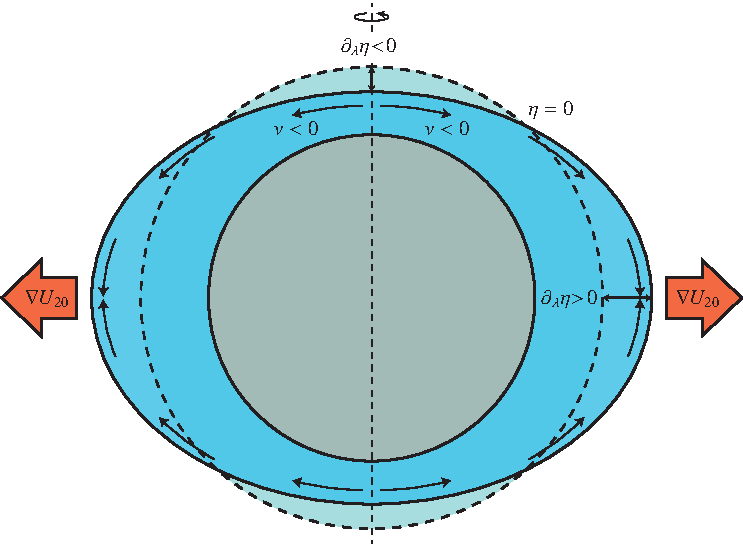
\includegraphics[width=\linewidth]{Figures/CoordProb}
\caption{Schematic representation of the ocean tide due to the eccentricity-radial tidal potential ($U_{20}$), at periapsis. Taking a derivative of $v$ across the north pole yields a null result in the spherical coordinate system, despite the clear mass divergence away from the poles leading to $\eta < 0$.\label{fig:coord_prob}}
\end{figure}

Add flow chart?

A natural issue arising from the choice of grid is the time step used. As described in section \ref{subsec:grid}, the fixed latitude-longitude grid causes meridian lines to converge at the pole. Nodes near the pole therefore have much smaller spatial sperations than those at the equator. As a result, in order to satisfy the Courant-Friedrichs-Lewy (CFL) condition required for numerical stability, $\Delta t \lesssim 40 \si{\second}$ if $\Delta \lambda = \Delta \phi = 4^{\circ}$ \citep{arakawa1977computational,sears1995tidal}. This massive constraint on the time step is often referred to as the ``pole problem''. Several workarounds to ease the time step have been applied throughout the literature \citep{comblen2009finite}. For example, it is common to apply a fourier filter to remove high wavenumber components of the solvable fields near the poles \citep{murray2002fourier}, or to use the spectral transform method as reviewed by \citet{swarztrauber1996spectral}. In this work, however, we apply none of these methods, and obey the CFL condition by selecting the appropriate time step for the model resolution.

A more significant issue arises from the combined choice of coordinate system and grid structure. Nodes located directly at the pole become singularities in space, where the normal directions east and west used to define the velocity components suddenly become meaningless. Consider the northward velocity flow near the north pole under the eccentricity-radial tide, shown in Figure \ref{fig:coord_prob}. Conservation of mass and the formation of an equatorial bulge force flow to diverge away from the pole. To solve for the surface displacement node directly at $\lambda = 90^{\circ}$, we must take the derivative of $v$ across the pole (as in Equation \ref{eq:momv_fd}). As each $v$ node located either side of the pole has the same magnitude and, perhaps unintuitively, is orientated in the same direction (southwards), this derivative becomes zero. As the derivative of $u$ in Equation \ref{eq:momu_fd} is also zero, we find that surface displacment at the pole must become zero as well. Yet, as there is divergence away from the pole, it is required that $\eta < 0$ to conserve mass. Clearly, the choice of coordinate system and grid do not permit such behaviour at the poles. 

To workaround this problem, we employ one dimensional quadratic Lagrangian interpolation for all $u$ and $\eta$ nodes located at the pole, consequently avoiding having to directly solve for these points. We then take the mean of the interpolated points, and prescribe that as the polar values. The interpolation obviously works better for higher grid resolutions, so for the deepest oceans we are forced to decrease $\Delta \lambda$ and $\Delta \phi$ to maintain pole stability. This is turn forces a greater constraint on the model's time step.

\subsection{Model Setup and Parameters \label{subsec:param}}



All numerical results presented in the following section are for surface oceans on Titan, as was the case for \citet{sears1995tidal,sohl1995tidal}. This is an appropriate benchmark for our numerical model because, as already discussed, we base much of the numerical scheme on that described by \citet{sears1995tidal} who also applied his model to Titan.

The main parameters used in our simulations are given in table 1. We first perform both semi-analytical and numerical simulations for the ``canonical'' ocean depth of $h=400 \, \si{\metre}$ \citep{sagan1982tide,sears1995tidal}. These simulations assume Rayleigh friction, providing us with a means of testing the numerical results against the analytical solutions. We assume \hbox{$\alpha = 2.28 \times 10^{-7} \, \si{\per\second}$}, corresponding to a tidal $Q$ of $10$ \citep{tyler2011tidal}. A simulation is run for both the eccentricity and obliquity tides. Additionally, the numerical solution to the full tidal potential (Equation \ref{eq:U_2}) is also run. This is not possible analytically, so solutions are instead superimposed together. Comparisons are made between $\bm{u}$, $\eta$ and $\left\langle F_\alpha \right\rangle_{orbit}$ for these test cases and the analytical solutions. 

Following comparison of these individual cases, we then compare the orbitally averaged dissipation between the numerical and analytical solutions across a large parameter space in $h$ and $\alpha$ space. Solutions over this kind of parameter space are what revealed the dissipative resonances first described and discovered by \citet{tyler2011tidal}, providing another excellent test case for our numerical model.

\begin{table}[!t]
\scriptsize
\centering
\begin{tabularx}{\linewidth}{p{1.8cm} p{2cm} p{1cm} p{1.2cm}}
 \toprule
Parameter & Description & Titan & Enceladus\\
 \midrule \midrule
$\Omega$ [$\times 10^{-5}$ \si{\radian\per\second}]	& angular velocity 		& $0.455$ & $5.31 $ \\
$r$ [\si{\kilo\metre}]				& satellite radius 		& $2574.7$ & $252.1$\\
$a$ [$\times 10^6$ \si{\kilo\metre}]				& semi-major axis 		& $1.221865$ & $0.238042$\\
$g$ [\si{\metre\per\second\squared}]		& surface gravity 		& $1.35$ & $0.11$\\
$e$ 								& eccentricity 			& $0.0288$ & $0.0044$\\
$-\theta_0$ [$^{\circ}$] 			& obliquity 			& $0.32$ & $0.0027$\\
$k_2$ 								& tidal Love number 	& $0.120$ & $0.0010$\\
$h_2$ 								& tidal Love number 	& $0.221$ & $0.0017$\\
 \bottomrule
\end{tabularx}
\caption{Model parameters used in all simulations presented here. All values are specific to Titan, and are taken from \citet{zebker2009size,chen2013tidal}.  \label{tb:param}}
\end{table}

In the final series of simulations Rayleigh friction is replaced by bottom friction. Again, orbitally averaged dissipation was explored over a large parameter range, but this time in $h$, $c_D$ space. This allows us to investigate how the addition of bottom friction affects the ocean dissipation resonances. 
